%%%%%%%%%%%%%%%%%%%%%%%%%%%%%%%%%%%%%%%%%%%%%%%%%%%%%%%%%%%%%%%%%%%%%%%%%%%%%%%%
%2345678901234567890123456789012345678901234567890123456789012345678901234567890
%        1         2         3         4         5         6         7         8

\documentclass[letterpaper, 10 pt, conference]{ieeeconf}  % Comment this line out
                                                          % if you need a4paper
%\documentclass[a4paper, 10pt, conference]{ieeeconf}      % Use this line for a4
                                                          % paper
\usepackage[english]{babel}
\usepackage[utf8]{inputenc}
\usepackage{amsmath}
\usepackage{blindtext}
\usepackage{scrextend}
\usepackage{fontawesome5}
\usepackage{graphicx}
\usepackage{hyperref}
\usepackage{enumitem}
\usepackage{enumerate}
\usepackage{upgreek}
\usepackage{listings}
\usepackage{amssymb}
\usepackage[export]{adjustbox}
\usepackage[colorinlistoftodos]{todonotes}
\IEEEoverridecommandlockouts                              
\overrideIEEEmargins

\definecolor{codegreen}{rgb}{0,0.6,0}
\definecolor{codegray}{rgb}{0.5,0.5,0.5}
\definecolor{codepurple}{rgb}{0.58,0,0.82}
\definecolor{backcolour}{rgb}{0.95,0.95,0.92}

\lstdefinestyle{mystyle}{
    backgroundcolor=\color{backcolour},   
    commentstyle=\color{codegreen},
    keywordstyle=\color{magenta},
    numberstyle=\tiny\color{codegray},
    stringstyle=\color{codepurple},
    basicstyle=\ttfamily\footnotesize,
    breakatwhitespace=false,         
    breaklines=true,                 
    captionpos=b,                    
    keepspaces=true,                 
    numbers=left,                    
    numbersep=5pt,                  
    showspaces=false,                
    showstringspaces=false,
    showtabs=false,                  
    tabsize=2
}

\lstset{style=mystyle}

\title{\LARGE \bf
ZKU – Cohort 4 (Jul-Aug 2022)\\Week 3: More Circom\\Assignment \sharp 3}

% \author{Iskander Andrews\\\faIcon{discord} Isk#0996}
\author{Iskander Andrews$^{1}$% <-this % stops a space
\thanks{\noindent\rule{3cm}{0.4pt}}
\thanks{\faIcon{discord} \tt\small Isk#0996}
\thanks{\faIcon{twitter} \tt\small \href{https://twitter.com/iskdrews}{twitter.com/iskdrews}}
\thanks{\faIcon{github} \tt\small \href{https://github.com/iskdrews}{github.com/iskdrews}}
\thanks{\faIcon{linkedin} \tt\small \href{https://www.linkedin.com/in/iskander-andrews-99638313a/}{in/iskander-andrews}}
\thanks{\faIcon[regular]{envelope} \tt\small iskander.s.andrews@gmail.com}
}

\begin{document}



\maketitle
\thispagestyle{empty}
\pagestyle{empty}


%%%%%%%%%%%%%%%%%%%%%%%%%%%%%%%%%%%%%%%%%%%%%%%%%%%%%%%%%%%%%%%%%%%%%%%%%%%%%%%%
\begin{abstract}

This document is for answering ZKUC04, Week-1, Introduction to ZKP Assignment.
It consists of three main parts.
\begin{labeling}{alligator}
\item [\textbf{Part 1:}] Part 1 Circom in games.
\item [\textbf{Part 2:}] Part 2 Anti-collusion and Fairness.
\item [\textbf{Part 3:}] Part 3 Time to start thinking about your final project!.
\end{labeling}

The total number of questions and points is $6$, including the bonus questions. 
\end{abstract}

\noindent\rule{8cm}{0.4pt}

\section{\textbf{\underline{Part 1:}} Circom in games}
\subsection{\textbf{\underline{Question (1)}}}
\subsubsection{\textbf{\underline{1.1}  What have the authors done in their implementations to protect them from brute-force attacks?}}

Authors have used the idea of hashing the of the actual solution and the expected solution each of them with a random salt string, so that not revealing the actual solution.  

\noindent\rule{8cm}{0.4pt}

\section{\textbf{\underline{Part 2:}} Anti-collusion and Fairness}
\subsection{\textbf{\underline{Question (1)}}}
\subsubsection{\textbf{\underline{2.1.1} Summarize how MACI works in 2-4 sentences of simple English.}}

MACI that help developers to build a collusion-resistant applications, it is a bunch of smart-contracts and ZK circuits, so developers can build voting like applications. It provides important properties: 

\begin{itemize}
    \item Collusion resistance: where no-one can validate the vote except the trusted coordinator, so that breaks the effect of the briber. 
    \item Privacy: where no-one can decrypt the votes except the trusted coordinator.
    \item Uncensorability: where no-one event the trusted coordinator can censor the voting process. \cite{c1}
\end{itemize}

\subsubsection{\textbf{\underline{2.1.2} What kind of collusion(s) does MACI solve?}}
\begin{itemize}
    \item MACI is important the Decentralized Autonomous Organisations (DAOs) that govern through token voting system, because it protect against bribery attacks. 
\end{itemize}

\subsubsection{\textbf{\underline{2.1.3} What kind of collusion(s) or attack(s) does MACI not solve?}}
\begin{itemize}
    \item A key-selling attack, where recipient is inside a multisig, or inside trusted hardware.
    \item An attack where the original key is stored inside a trusted hardware which prevents key changes unless if it is a key known by an attacker. 
\end{itemize}
\subsection{\textbf{\underline{Question (2)}}}
\subsubsection{\textbf{\underline{2.2} Attach a screenshot of the tests passing in your PDF file.}}

\begin{figure}[htp]
    \centering
    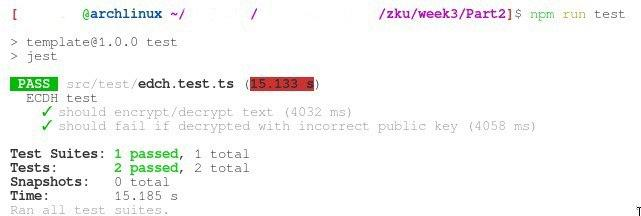
\includegraphics[width=9cm]{assets/photo_2022-07-25_23-23-16}
    \caption{All tests are passing.}
    \label{fig:galaxy}
\end{figure}

\subsection{\textbf{\underline{Question (3)}}}
\subsubsection{\textbf{\underline{4.1} Explain in 1-3 sentences why, in computing VDFs, having many computers operating in parallel won't help you to find the solution more quickly.}}

VDF function is sequential functions, which anyone can compute $f(x)$ in $t$ sequential steps. Therefore, it is impossible to speed up the computation with parallelism, because in case of the computation of some hash function $h$ that takes $t$ steps, the calculation of each application of the hash depends entirely on the output of the previous one. \cite{c2}

\noindent\rule{8cm}{0.4pt}

\section{\textbf{\underline{Part 3:}} Time to start thinking about your final project!}

\subsection{\textbf{}\underline{Question (1)}}
\subsubsection{\textbf{Suppose you are building a ZK \href{https://en.wikipedia.org/wiki/First-price_sealed-bid_auction}{blind auction} application and the circuit is already built for you. Write down an implementation plan, including what other components you will need to build, the order in which you will build your components, as well as what frameworks/tools you will use.}}

It depends on what is implemented in the circuit it-self, but I assume that the Circom circuit will be responsible for taking all the bids from the players in a private signal inputs, and then it compares until it outputs the greater one. And we could use Solidity contract to verify that selection, also we will need to implement a client application with React.js to allow users to connect to the circuit and the contract.

\subsection{\textbf{\underline{Question (2)}}}
\subsubsection{\textbf{Suggest three candidate ideas for your final project. Explain (1) the problem tackled, (2) a design overview, and (3) obstacles anticipated in approx. 200 words for each idea.}}

\begin{enumerate}[I.]
\item zkNerdle:
    \begin{enumerate}
        \item The problem tracked is a variation of the Wordle game, and it will use zkp to prove that the player knows the mathematical equation without revealing the equation to the verifier.
        \item The design would be by forking a front-end repo: \href{https://github.com/ayushpaharia/Nerdle}{\underline{github.com/ayushpaharia/Nerdle}}, and forking a zkp repo: \href{https://github.com/nalinbhardwaj/zordle}{\underline{github.com/nalinbhardwaj/zordle}} for the main Wordle game to refactor Halo2 circuits to fit Nerdle game rules.   
        \item The challenge is to understand more how to implement circuits on Halo2 which is written with Rust.
    \end{enumerate}
\item zkSuguru
    \begin{enumerate}
        \item The problem tracked is a variation of the Sudoku game, and it is about how to prove that the winner solved the puzzle without revealing the solution.
        \item The design would be by forking a front-end repo: \href{https://github.com/spassvogel/suguru}{\underline{github.com/spassvogel/suguru}} and will build the ZK circuit based on what I learnt on Assignment (1) on zkSudoku circuit.
        \item The challenges might be on testing the circuit with many different variation of the game. 
    \end{enumerate}
\item zkMinesweeper
    \begin{enumerate}
        \item The problem tackled is to prove that the winners cleared the rectangular board without clicking on any of the hidden "mines". 
        \item The design would be by forking a front-end repo: \href{https://github.com/kevin940726/minesweeper}{\underline{github.com/kevin940726/minesweeper}}, and then will implement the zkCircuit from scratch. 
        \item The challenge might be how to make sure that the ZK proof circuit is generalized for all the variation of the game. 
    \end{enumerate}
\end{enumerate}

\noindent\rule{8cm}{0.4pt}

\section*{ACKNOWLEDGMENT}
I would like to thank so much Heather @Giveth who told me to register in this great course, and would like to thank hadzija#0842 and cs#6500 for their great help and support. I am really thankful to them to everyone working behind the science to create, maintain, review, manage, and produce this great ZKP course, I see great efforts. 

\noindent\rule{8cm}{0.4pt}
\begin{thebibliography}{99}
\bibitem{c1} Koh Wei Jie, Oct 12, 2021, Release Announcement: MACI 1.0
 \href{https://medium.com/privacy-scaling-explorations/release-announcement-maci-1-0-c032bddd2157}{\underline{link}}
\bibitem{c2} Introduction to Verifiable Delay Functions (VDFs), OCTOBER 12, 2018 \href{https://blog.trailofbits.com/2018/10/12/introduction-to-verifiable-delay-functions-vdfs/}{\underline{link}}
\end{thebibliography}

\end{document}